\section{Performance Modeling}
\label{sec:performance-modeling}

In this section we describe the performance model used to analyze the target system. We will follow the widely adopted modeling approach suggested in \cite{leemis2006discrete}, which consists in (i) goals and objectives (ii) conceptual model (iii) specification model (iv) computational model (v) verification and (vi) validation.


% %
% GOALS AND OBJECTIVES
% %
\subsection{Goals and Objectives}
The main goals of simulation are about the system insights in terms of performance metrics.
%
In particular, considering $S=N$ we propose to evaluate system stationary and the following performance metrics with a $95\%$ level of confidence:

\begin{itemize}
	\item \textit{system response time} both global and per-class;
	
	\item \textit{response time} both global and per-class;
	
	\item \textit{Cloud response time} both global and per-class;
	
	\item \textit{system throughput} both global and per-class;
	
	\item \textit{Cloudlet throughput} both global and per-class;
	
	\item \textit{Cloud throughput} both global and per-class;
	
	\item \textit{interruption percentage} of the $2^{nd}$ class tasks;
	
	\item \textit{response time of interrupted tasks};
	
	\item \textit{system mean population} both global and per class;
	
	\item \textit{Cloudlet mean population} both global and per class;
	
	\item \textit{Cloud mean population} both global and per class;
	
	\item \textit{distribution of Cloudlet throughput} in terms of distribution fitting and cumulative distribution function.

\end{itemize}


% %
% CONCEPTUAL MODEL
% %
\subsection{Conceptual Model}
The conceptual model of the target system is the middle-level abstraction that makes the high-level architecture closer to the analytical model. We consider the conceptual model depicted in Figure~\ref{fig:conceptual-model}.

\begin{figure}
	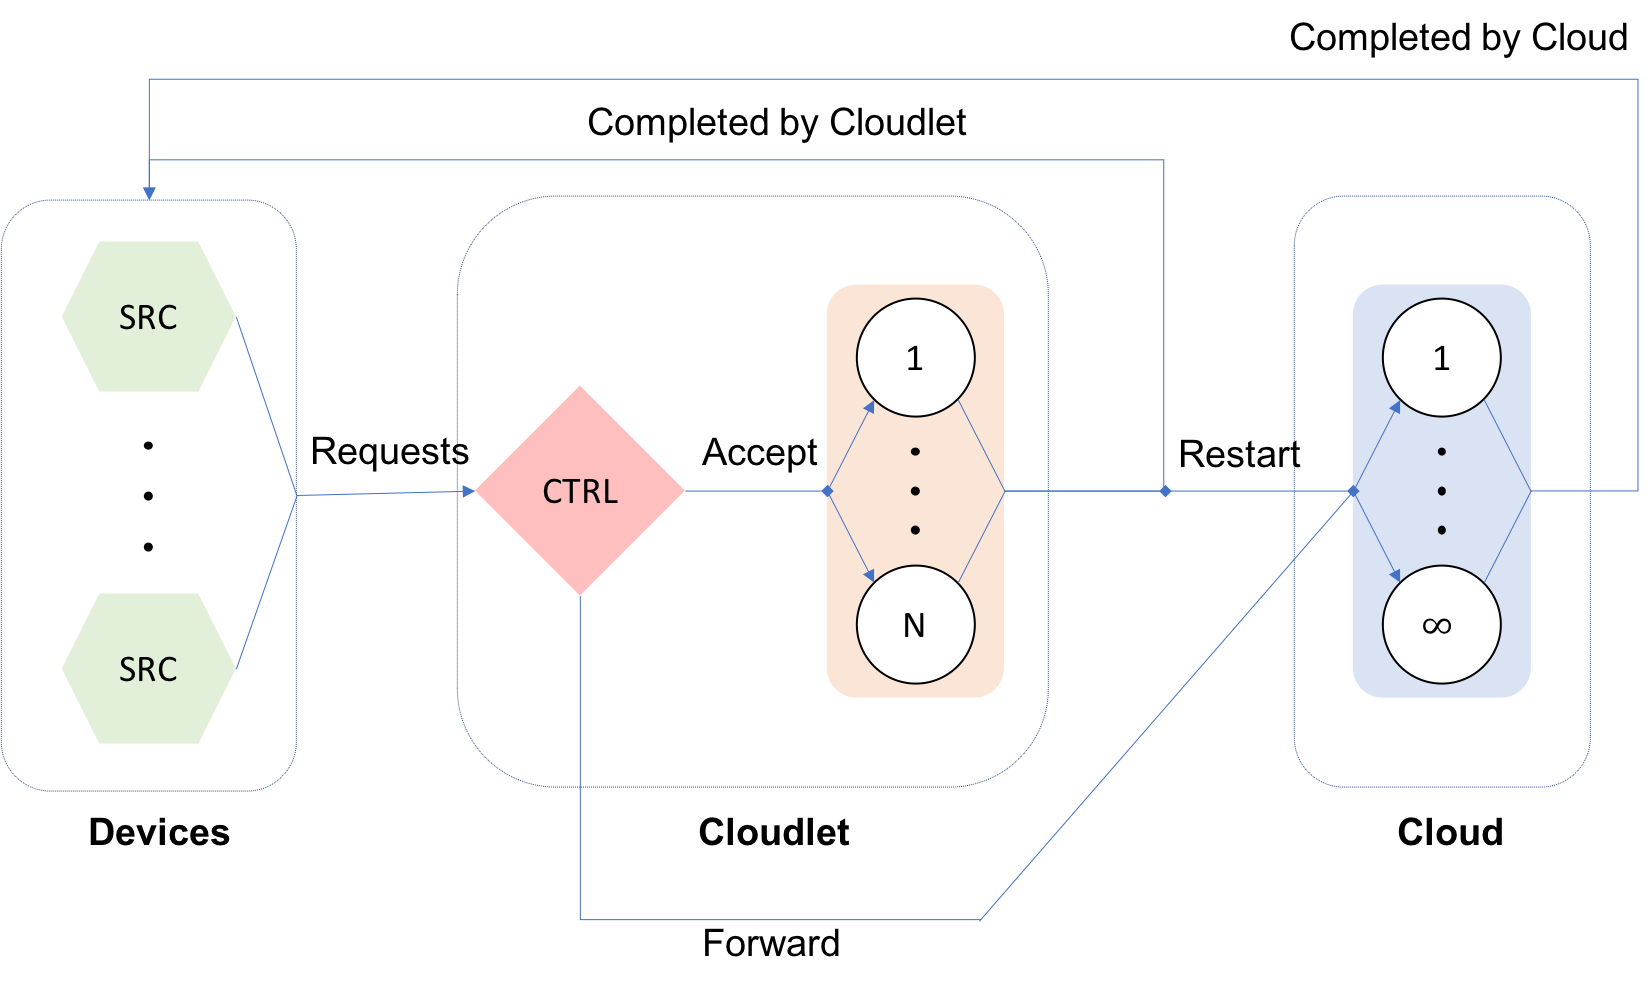
\includegraphics[width=\columnwidth]{fig/conceptual-model}
	\caption{Conceptual model.}
	\label{fig:conceptual-model}
\end{figure}

\paragraph{State space}
The state space $S$ of a system is a comprehensive characterization of the system. Each state $s \in S$ is a comprehensive characterization of the system in a given instant of time.
The state space of the whole system is represented by the state space of its subsystems:

\begin{itemize}
	\item \textit{Cloudlet}: $S_{clt} := \{(n_{clt,1},n_{clt,2})\in \mathcal{N}^{2}: n_{clt,1}+n_{clt,2}\leq N\}$, where $n_{clt,j}$ is the population of tasks belonging to the $j$-th class within the Cloudlet.
	
	\item \textit{Cloud}: $S_{cld} := \{(n_{cld,1},n_{cld,2})\in \mathcal{N}^{2}\}$, where $n_{cld,j}$ is the population of tasks belonging to the $j$-th class within the Cloud.
\end{itemize}

\paragraph{Events space}
An event is an occurrence that could change the state of the system at the event time, according to the event type.
We consider the following events:

\begin{itemize}
	\item $A_{clt,j}$: a task belonging to the $j$-th class arrives to the Cloudlet.
	
	\item $A_{cld,j}$: a task belonging to the $j$-th class arrives to the Cloud.

	\item $C_{clt,j}$: a task belonging to the $j$-th class is completed by the Cloudlet.
	
	\item $C_{cld,j}$: a task belonging to the $j$-th class is completed by the Cloud.
	
	\item $R_{2}$: a task belonging to the $2^{nd}$ class is interrupted in the Cloudlet and restarted in the Cloud.
\end{itemize}

% %
% SPECIFICATION MODEL
% %
\subsection{Specification Model}
The typical modeling workflow requires to specify
(i) the statistical analysis of data collected from the real system in order to determine the input model to drive simulations,
(ii) the adopted simulation approach,
(ii) the algorithms involved in computations and
(iii) the analytical model and equations to determine performance metrics.

Given the importance of the analytical model, we reserve a dedicated section for discussing about it.

Regarding the simulation approach, we decided to adopt the \textit{next-event simulation method}, which is the most effective discrete-event method in terms of algorithmic modeling, time management and computational requirements.

\paragraph{Statistical specifications}
In our case we have been provided with the statistical characterization of the target system.
Tasks belonging to the $j$-th class arrive to the system according to an exponential arrival process with rate $ \lambda_{j}$.
The Cloudlet serves tasks belonging to the $j$-th class according to an exponential service process with rate $\mu_{clt,j}$; the Cloud serves tasks belonging to the $j$-th class according to an exponential service process with rate $\mu_{cld,j}$.
We assume that 
(i) $\mu_{clt,i}>\mu_{cld,i}\ \forall i=1,2$ and
(ii) the setup time $T_{setup}$ is exponentially distributed with expected value $E[T_{setup}]$.

In particular, we consider values shown in Equations~\ref{eqn:statistical-specifications}.

\begin{equation} 
\begin{split}
\lambda_{1}  &=6.00\;tasks/sec \\
\lambda_{2}  &=6.25\;tasks/sec \\
\mu_{clt,1}  &=0.45\;tasks/sec \\
\mu_{clt,2}  &=0.27\;tasks/sec \\
\mu_{cld,1}  &=0.25\;tasks/sec \\
\mu_{cld,2}  &=0.22\;tasks/sec \\
E[T_{setup}] &=0.8\;sec \\
\end{split}
\label{eqn:statistical-specifications}
\end{equation}

\paragraph{Algorithmic specifications}
From the point of view of algorithms involved in the simulation, we need to specify:

\begin{itemize}
	
	\item \textit{off-loading algorithm}, which defines the off-loading policy implemented by the \textit{Cloudlet controller (CTRL)}, as defined in Algorithm~\ref{alg:offloading-policy}.
	
	\item \textit{simulation algorithm}, which defines the main execution flow of the simulator, as defined in Algorithm~\ref{alg:simulation}.
\end{itemize}

With reference to the simulation algorithm, we need to focus on the following aspects:

\begin{itemize}
	
	\item \textit{arrival generation}: a new random arrival is generated every time an arrival is processed. As we need to submit classed arrival, we adopted Algorithm~\ref{alg:arrivals} whose statistical correctness relies on the properties of the exponential distribution.
	
	\item \textit{event submission}: when a new event is submitted to the system, system components (i) updates both their state (ii) update simulation counters and (iii) generate a random response event, i.e. completion event or an interruption event.
	
	\item \textit{stop condition}: when this condition holds true, the simulation is terminated. In particular, the logical definition is twofold:
	When the simulator is used for transient analysis, the condition holds true when the simulation clock is greater than the stop time.
	When the simulator is used for performance analysis, the condition holds true when the closed-door condition does and the system has reached the idle state.
	
	\item \textit{closed-door condition}: when this condition holds true, no more arrivals will be generated and system will only handle remaining completion until its state reaches the initial idle condition.
	
	\item \textit{sampling condition}: when this condition holds true, performance metrics should be sampled.
	
	\item \textit{metrics management}: when the system handles an event, it updates simulation counters, e.g. number of arrivals, service time, integral areas and so on. When the sampling condition holds true, those counters are used to opportunely computes a sample of performance metrics. Such a sample is used to update performance metrics collection, which leverages the \textit{one-pass Wellford algorithm, batch means and confidence intervals} using formulas specified in \cite{leemis2006discrete}.
\end{itemize}

\begin{algorithm}
	\SetAlgoLined
	\If{task of class 1}{
		\If{$n_{clt,1}=N$}{
			send to the Cloud
		} 
		\If{$n_{clt,1}+n_{clt,2}<S$}{
			accept on the Cloudlet
		} 
		\eIf{$n_{clt,2} > 0$}{
			accept on the Cloudlet, interrupt a $2^{nd}$ class task in the Cloudlet and restart it in the Cloud
		}{
			accept on Cloudlet
		}
	}
	\If{arrival of class 2}{
		\eIf{$n_{clt,1}+n_{clt,2}>=S$}{
			send to the Cloud
		}{
			accept on the Cloudlet
		}
	}
	\caption{Off-loading.}
	\label{alg:offloading-policy}
\end{algorithm}

\begin{algorithm}
	\SetAlgoLined
	
	calendar.schedule\_arrival();
	
	\While{$\neg stop\_condition()$}{
		e = calendar.next\_event();
		
		\If{$\neg close\_door\_condition() \vee e.type = completion$}{
			e\_next = submit\_event(e);
			
			calendar.schedule(e\_next);
		} 
		\If{$\neg close\_door\_condition() \vee e.type = arrival$}{
			calendar.schedule\_arrival();
		} 
		\If{$sampling\_condition()$}{
			sample = sampling();
			
			update\_metrics(sample);
		}
	}
\caption{Simulation.}
\label{alg:simulation}
\end{algorithm}

\begin{algorithm}
	\SetAlgoLined
	
	rndgen.stream(ARRIVAL)
	
	$p_{1}=\frac{\lambda_{1}}{\lambda_{1}+\lambda_{2}}$
	
	u = rndgen.uniform(0.0,1.0)
	
	\eIf{$u\leq p_{1}$}{
		arrival\_type = TASK\_1
		
		rndgen.stream(ARRIVAL\_TASK\_1)
		
		$t_{inter-arrival}$ = rndgen.exponential($\lambda_{1}$)
	}{
		arrival\_type = TASK\_2
		
		rndgen.stream(ARRIVAL\_TASK\_2)
		
		$t_{inter-arrival}$ = rndgen.exponential($\lambda_{2}$)
	}
	
	$t_{arrival}=t_{last\_arrival}+t_{inter-arrival}$

	$t_{last\_arrival}=t_{arrival}$
	
	schedule(arrival\_type,$t_{arrival}$)
	
	\caption{Arrivals generation.}
	\label{alg:arrivals}
\end{algorithm}

% %
% ANALYTICAL MODEL
% %
\subsection{Analytical Model}
In this Section we define and solve the \textit{analytical model} of the system.
%
In particular, we will first show the Markov Chain and flow balance equations for a very simple case, in order to introduce the reader to the structure of the chain with its critical states.
%
Then, we will cover the general case showing formulas of routing probabilities and performance metrics.
%
At the end, we will solve the target case explaining how we solve it.

The \textit{analytical model} is depicted in Figure~\ref{fig:analytical-model}, whose \textit{routing probabilities} are defined in Equation~\ref{eqn:routing-probabilities}.
The definition of routing probabilities relies on the following subsets of states $S_{clt,i} \subset S_{clt}$:

\begin{itemize}
	\item $S_{clt,1}$:  a task belonging to the $1^{st}$ class is accepted in the Cloudlet.
	
	\begin{equation}
	S_{clt,1} := \{(n_{clt,1},n_{clt,2})\in S_{clt} : n_{clt,1}+n_{clt,2}<N \vee n_{clt,2}>0\}
	\end{equation}
	
	\item $S_{clt,2}$: a task belonging to the $2^{nd}$ class is accepted in the Cloudlet.
	
	\begin{equation}
	S_{clt,2} := \{(n_{clt,1},n_{clt,2})\in S_{clt} : n_{clt,1}+n_{clt,2}<N \wedge n_{clt,2}<S\}
	\end{equation}
	
	\item $S_{clt,3}$: a task belonging to the $2^{nd}$ class is interrupted in the Cloudlet and it is restarted in the Cloud.
	
	\begin{equation}
	S_{clt,3} := \{(n_{clt,1},n_{clt,2})\in S_{clt} : n_{clt,1}+n_{clt,2}=N \wedge n_{clt,2}>0\}
	\end{equation}
\end{itemize}

\begin{figure}
	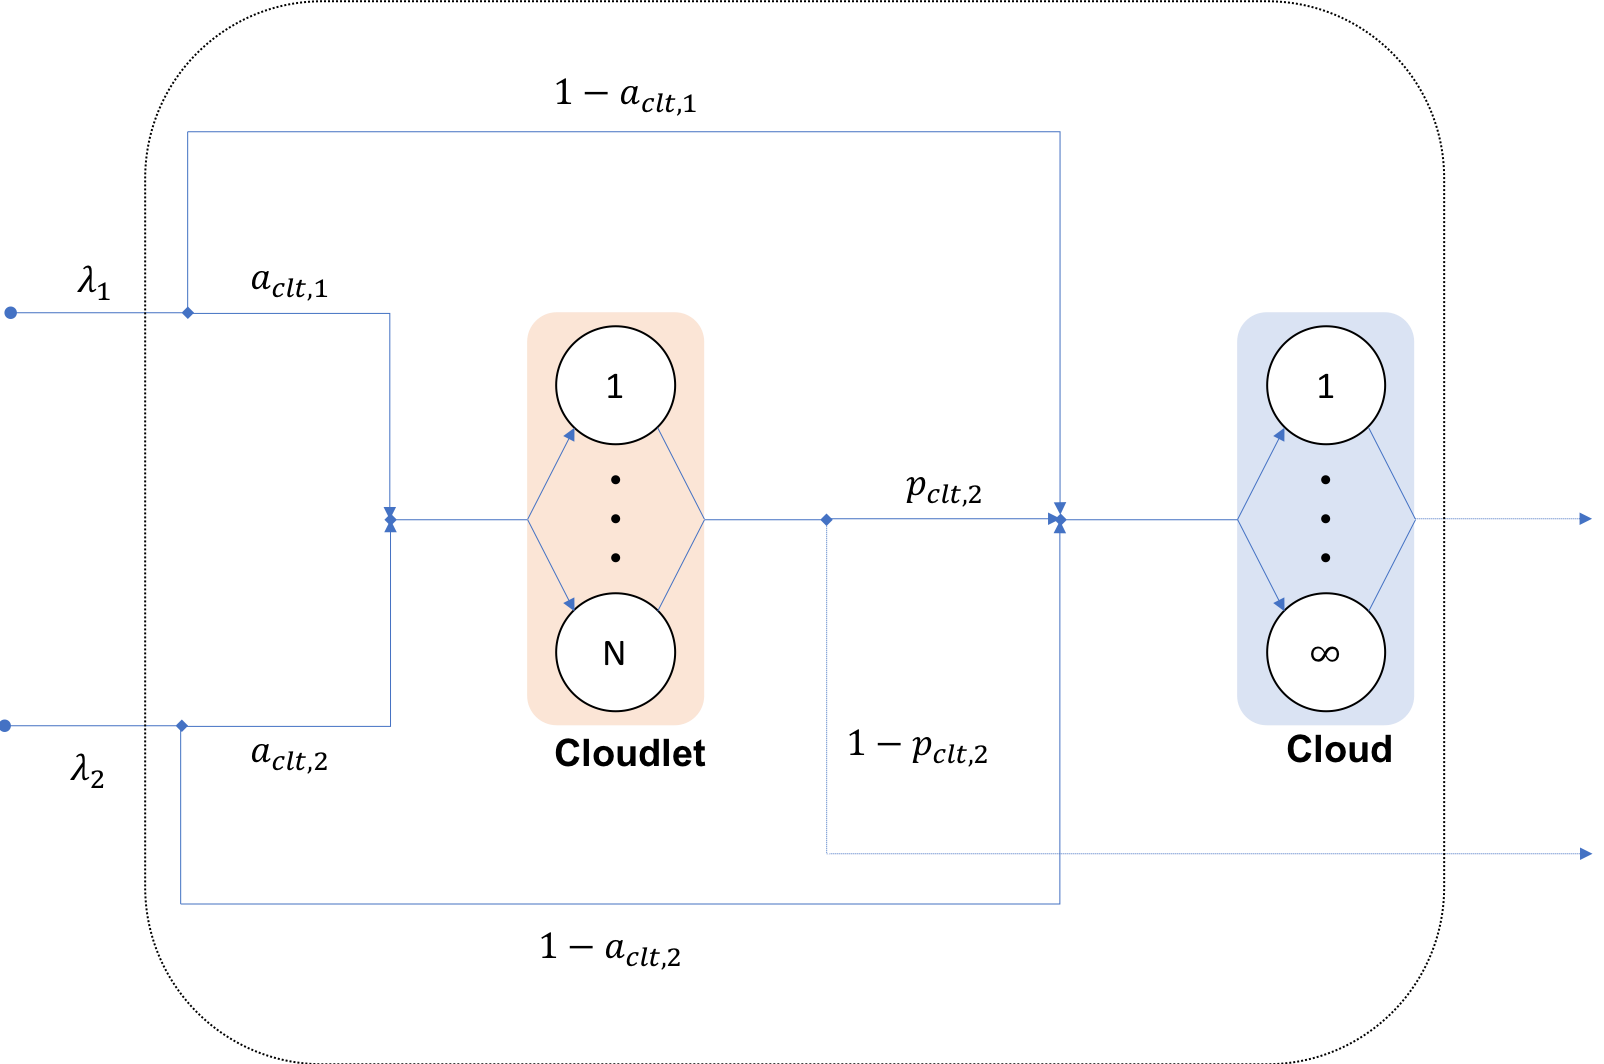
\includegraphics[width=\columnwidth]{fig/analytical-model}
	\caption{Analytical model.}
	\label{fig:analytical-model}
\end{figure}

\begin{equation} 
\begin{split}
a_{clt,1} & = \sum_{s\in S_{clt,1}} \pi_{s} \\
a_{clt,2} & = \sum_{s\in S_{clt,2}} \pi_{s} \\
r_{clt,2} & = \sum_{s\in S_{clt,3}} \pi_{s} \Big(\frac{\lambda_{2}}{\lambda_{1}+\lambda_{2}}\Big) \\
\end{split}
\label{eqn:routing-probabilities}
\end{equation}


\paragraph{Markov Chain}
Assuming Poisson arrivals and exponential services, we can determine the Markov Chain whose resolution allows us to compute the routing probabilities shown in Equation~\ref{eqn:routing-probabilities}.

In Figure~\ref{eqn:analytical-model-markov} we show the Markov Chain with the associated flow balance equations listed in Equation~\ref{eqn:analytical-model-markov}.
For sake of simplicity, we consider here the simple case with $N=S=2$ in order to (i) give an idea of the system of equations to be solved and (ii) graphically recognize the critical states. In fact, the representation fo the Markov Chain and the associated equations would be inpractical for the case $N=S=20$, due to the combinatorial explosion of the state space.

In the considered simple case, the critical states are:

\begin{itemize}
	\item $(2,0)$: every arrival is forwarded to the Cloud;
	
	\item $(1,1)$: every arrival belonging to class 1 is accepted in Cloudlet, causing the restart in Cloud of the serving task belonging to class 2; whilst every arrival belonging to class 2 is forwarded to Cloud;
	
	\item $(0,2)$: every arrival belonging to class 1 is accepted in Cloudlet, causing the restart in Cloud of a random serving task of Class 2; whilst every arrival belonging to class 2 is forwarded to Cloud;
\end{itemize}

\begin{figure}
	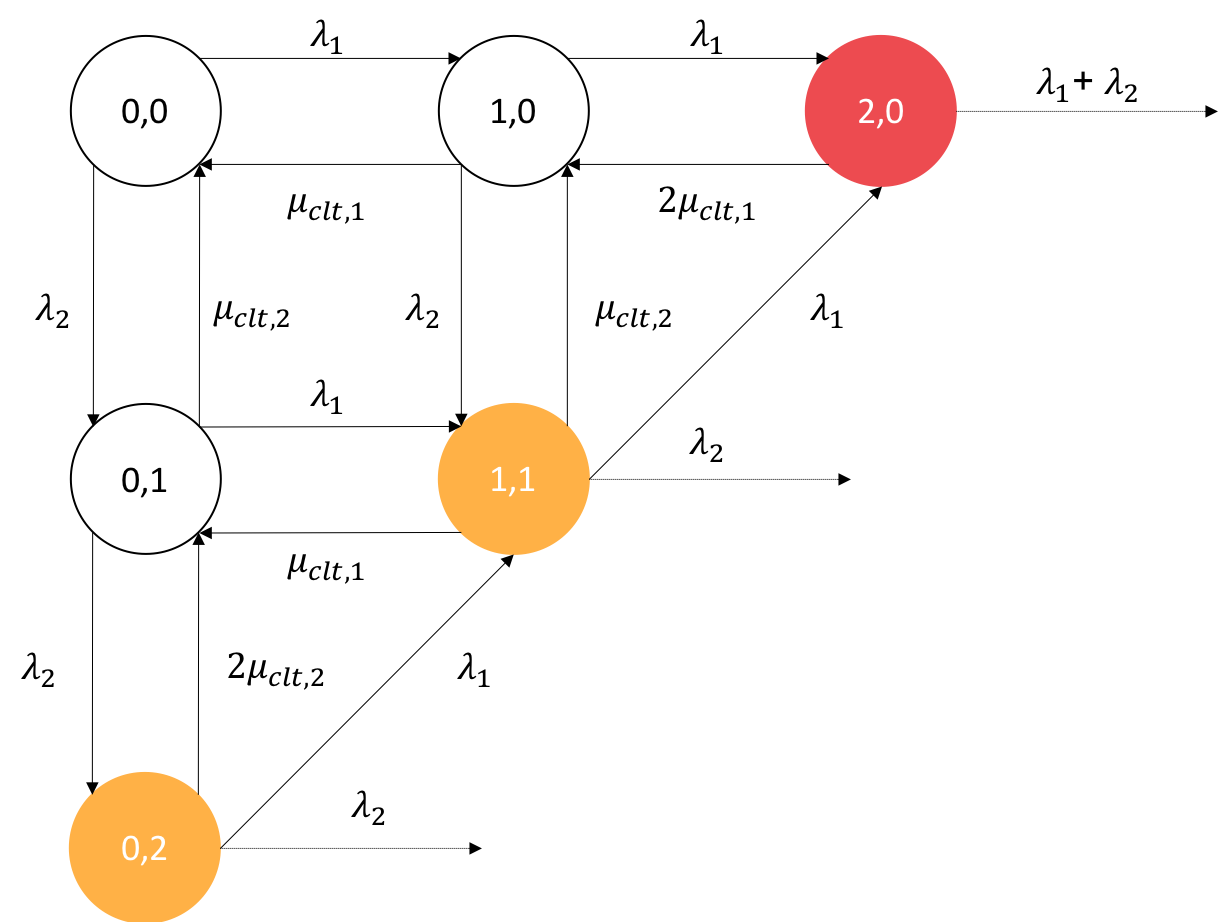
\includegraphics[width=\columnwidth]{fig/analytical-model-markov}
	\caption{Markov Chain with $N=2$ and $S=2$.}
	\label{fig:analytical-model-markov}
\end{figure}

\begin{equation} 
\begin{split}
\pi_{0,0}(\lambda_{1}+\lambda_{2})& = \pi_{1,0}\mu_{clt,1}+\pi_{0,1}\mu_{clt,2} \\
\pi_{0,1}(\lambda_{1}+\lambda_{2}+\mu_{clt,2}) & = \pi_{0,0}\lambda_{2}+\pi_{1,1}\mu_{clt,1}+\pi_{0,2}2\mu_{clt,2} \\
\pi_{1,0}(\lambda_{1}+\lambda_{2}+\mu_{clt,1}) & = \pi_{0,0}\lambda_{1}+\pi_{1,1}\mu_{clt,2}+\pi_{2,0}2\mu_{clt,1} \\
\pi_{1,1}(\lambda_{1}+\mu_{clt,1}+\mu_{clt,2}) & = \pi_{0,1}\lambda_{1}+\pi_{1,0}\lambda_{2}+\pi_{0,2}\lambda_{1} \\
\pi_{0,2}(\lambda_{1}+2\mu_{clt,2}) & = \pi_{0,1}\lambda_{2} \\
\pi_{2,0}2\mu_{clt,1} & = \pi_{1,0}\lambda_{1}+\pi_{1,1}\lambda_{1} \\
1 & = \pi_{0,0}+\pi_{0,1}+\pi_{1,0}+\pi_{1,1}+\pi_{0,2}+\pi_{2,0}\\
\end{split}
\label{eqn:analytical-model-markov}
\end{equation}

\paragraph{Accepted Workload}
Given the routing probabilities we can determine the following \textit{accepted workloads}:

\begin{itemize}
	\item \textit{Cloudlet}: arrival rate of tasks belonging to $j$-th class accepted in Cloudlet:
	\begin{equation}
	\lambda_{clt,j} = a_{clt,j}\lambda_{j}
	\end{equation}
	
	\item \textit{Cloud}: arrival rate of tasks belonging to $j$-th class forwarded to Cloud:
	\begin{equation}
	\lambda_{cld,j} = (1-a_{clt,j})\lambda_{j}
	\end{equation}
	
	\item \textit{Restarts}: rate of tasks belonging to $2^{nd}$ class interrupted in Cloudlet and restarted in Cloud:
	\begin{equation}
	\lambda_{r} = r(\lambda_{1}+\lambda_{2})
	\end{equation}
\end{itemize}

\paragraph{Performance metrics}
Given the accepted workloads we can determine the following \textit{performance metrics for classed tasks in each subsystem}.
%
We assume here to know the expected time lost in Cloudlet by $2^{nd}$ class tasks before their interruption. In particular, as we are not able to determine $E[T_{clt,2,lost}]$ from the Markov Chain, we will assume the experimental value computed by the simulator.

\begin{itemize}
	\item $1^{st}$ class in Cloudlet:
	\begin{equation} 
	\begin{split}
	E[T_{clt,1}] &= \frac{1}{\mu_{clt,1}} \\
	E[N_{clt,1}] &= \lambda_{clt,1}E[T_{clt,1}] \\
	\end{split}
	\end{equation}

	\item $2^{nd}$ class in Cloudlet:
	\begin{equation} 
	\begin{split}
	E[T_{clt,2}] &= \frac{1}{\mu_{clt,2}} \\
	E[N_{clt,2}] &= \lambda_{clt,2}E[T_{clt,2}]-\lambda_{r} E[T_{clt,2,lost}] \\
	\end{split}
	\end{equation}
	
	\item $1^{st}$ class in Cloud:
	\begin{equation} 
	\begin{split}
	E[T_{cld,1}] &= \frac{1}{\mu_{cld,1}} \\
	E[N_{cld,1}] &= \lambda_{cld,1}E[T_{cld,1}] \\
	\end{split}
	\end{equation}
	
	\item $2^{nd}$ class in Cloud (not restarted):
	\begin{equation} 
	\begin{split}
	E[T_{cld,2}]^{[NR]} &= \frac{1}{\mu_{cld,2}} \\
	E[N_{cld,2}]^{[NR]} &= \lambda_{cld,2}E[T_{cld,2}]^{[NR]} \\
	\end{split}
	\end{equation}
	
	\item $2^{nd}$ class in Cloud (restarted):
	\begin{equation} 
	\begin{split}
	E[T_{cld,2}]^{[R]} &= E[T_{setup}]+ E[T_{cld,2}]^{[NR]} \\
	E[N_{cld,2}]^{[R]} &= \lambda_{r}E[T_{cld,2}]^{[R]} \\
	\end{split}
	\end{equation}
	
	\item $2^{nd}$ class in Cloud (both restarted and not restarted):
	\begin{equation} 
	\begin{split}
	E[T_{cld,2}] &= \sum_{m=NR,R}\frac{E[N_{cld,2}]^{[m]}}{E[N_{cld,2}]}E[T_{cld,2}]^{[m]} \\
	E[N_{cld,2}] &= \sum_{m=NR,R}E[N_{cld,2}]^{[m]} \\
	\end{split}
	\end{equation}
\end{itemize}

Then we can determine the following \textit{performance metrics for each subsystem}:

\begin{itemize}
	\item Cloudlet:
	\begin{equation} 
	\begin{split}
	E[T_{clt}] &= \sum_{j=1,2}\frac{E[N_{clt,j}]}{E[N_{clt}]}E[T_{clt,j}] \\
	E[N_{clt}] &= \sum_{j=1,2}E[N_{clt,j}] \\
	E[X_{clt}] &= \sum_{j=1,2}\lambda_{clt,j}-\lambda_{r} \\
	\end{split}
	\end{equation}
	
	\item Cloud:
	\begin{equation} 
	\begin{split}
	E[T_{cld}] &= \sum_{j=1,2}\frac{E[N_{cld,j}]}{E[N_{cld}]}E[T_{cld,j}] \\
	E[N_{cld}] &= \sum_{j=1,2}E[N_{cld,j}] \\
	E[X_{cld}] &= \sum_{j=1,2}\lambda_{cld,j}+\lambda_{r} \\
	\end{split}
	\end{equation}
\end{itemize}

Finally, we can determine the following \textit{performance metrics for the whole system}:

\begin{equation} 
\begin{split}
E[T] &= \sum_{i=cld,clt}\frac{E[N_{i}]}{E[N]}E[T_{i}] \\
E[N] &= \sum_{i=cld,clt}E[N_{i}] \\
E[X] &= \sum_{i=cld,clt}E[X_{i}] \\
\end{split}
\end{equation}

Thinking about the \textit{utilization of each subsystem}, the following hold true:

\begin{itemize}
	\item Cloudlet: simplifying our argument by assuming the whole incoming traffic belonging to the $1^{st}$ class served at the maximum rate (the best case), we can state that
	\begin{equation} 
	\rho_{clt} = \frac{\lambda_{1}+\lambda_{2}}{N\mu_{clt,1}}\rightarrow 0
	\end{equation}
	That is, the Cloudlet is not able to serve all traffic as it saturates.
	
	\item Cloud: as a queue with infinite resources, we can conclude that
	\begin{equation}
	\rho_{cld} \rightarrow 0
	\end{equation}
	That is, the Cloud can handle all requests as it never saturates.
\end{itemize}


\paragraph{Resolution}
Given the \textit{analytical model} depicted in Figure~\ref{fig:analytical-model}, the resolution of the Markov Chain for the case $S=N=20$ allows us to determine routing probabilities and performance metrics.

We solved the the \textit{analytical model} depicted in Figure~\ref{fig:analytical-model} leveraging a \textit{Python script} that 
(i) receives as input the system configuration
(ii) generates the Markov Chain representing the Cloudlet
(iii) generates the system of equations from the Markov Chain
(iv) computes limiting probabilities by solving the system
(v) computes routing probabilities
(vi) computes performance metrics and
(vii) display a report of results.

Analytical results are presented in Figure~\ref{tbl:evaluation}, along with their experimental counterpart.
%
We preferred to present analytical and experimental results in a unique common view, in order to provide the reader with an idea on how the simulator approximates analytical results.


% %
% COMPUTATIONAL MODEL
% %
\subsection{Computational Model}
The proposed simulator has been designed following the \textit{next-event simulation} paradigm and has been implemented as a \textit{Python} application. The full open source code is available in a public Github repository \cite{gmarciani-pydes}.

\paragraph{Configuration}
The simulation parameters can be fully configured with a YAML file loaded when the simulator starts up. In particular, the following parameters can be configured:

\begin{itemize}
	\item \textit{arrival process}: the user can configure the statistical distribution law and parameters of arrivals for both task classes. In this work, we consider the Exponential distribution, but any statistical distribution can be set.
	
	\item \textit{service process}: the user can configure the statistical distribution law and parameters of services for both task classes. In this work, we consider the Exponential distribution, but any statistical distribution can be set.
	
	\item \textit{setup time}: the user can configure the statistical distribution law and parameters of the setup time for both task classes. In this work, we consider a Deterministic setup time set to zero for the $1^{st}$ class and an Exponential setup time for the $2^{nd}$ class, but any statistical distribution can be set.
	
	\item \textit{Cloudlet dimension}: the user can configure the number of Cloudlet resources.
	
	\item \textit{Cloudlet threshold}: the user can configure the threshold for the restart condition of $2^{nd}$ class tasks in the Cloudlet.
	
	\item \textit{server selection policy}: the user can configure the policy adopted to select the $2^{nd}$ class task to interrupt in the Cloudlet when the threshold has been reached. In this work, we consider the Random selection, but the user can choose among Random, Ordered, Cyclic and Equity selection policies.
\end{itemize}

\paragraph{Randomization}
Random components are ruled by a custom \textit{multi-stream Lehmer generator} to generate pseudo-random events, whose parameters have been described in Section~\ref{sec:random-number-generation} and whose evaluation is presented in Section~\ref{sec:evaluation}.
The \textit{degree of randomization} has been improved by associating the random component the following processes to a dedicated stream of the pseudo-random number generator: arrival process of each task class, service process of each servant and server selection rule.
This strategy has been motivated by the fact that in a real case scenario we can assume the independence between (i) inter-classed workload, (ii) computational offer of distinct resources and (iii) selection strategies.

\paragraph{Event management}
Events are managed by a \textit{priority-queue based calendar} with the ability both to schedule and un-schedule events.
%
Even if both the initial and terminal state can have any possible value, we adopted the convention of initializing and terminating the system in the idle state $(0,0,0,0)$. In particular, the terminal state is reached via the well-known closed door technique driven by a stop time condition.
%
The calendar is initialized by scheduling the first arrival in the initialization phase. The submission of an arrival $a$ to the system could induce
(i) the scheduling of the corresponding completion event,
(ii) the scheduling of a new arrival, or
(iii) the unscheduling of a previously scheduled completion, i.e. interruption in Cloudlet.
%
The next-event calendar is implemented as priority queue, appropriately extended to manage scheduling/unscheduling of events and exclusion of impossible events, i.e. arrivals with occurrence time greater than the stop time.
%
The impossibility of events is managed by letting the calendar contain possible events only, which is the best approach when the event list is assumed to be very long.

\paragraph{Software Classes}
We provide here a short description of the main software classes involved in our simulator, in order to help the reader navigate through our code.

\begin{itemize}

	\item \textit{Simulation}: simulator entry-point, responsible to load and validate configurations, create the calendar of events, the statistics and the target system, show the real-time progress of the simulation, determine the duration of the simulation, write sampling files, reports and output results.
	
	\item \textit{Calendar}: calendar of events, implemented as a priority-queue with the ability to both schedule and unschedule events.
	
	\item \textit{System}: high level abstraction of the whole system, responsible to initialize the Cloudlet, initialize the Cloud, implement the Controller logic and update system-level classed/global metrics.
	
	\item \textit{Cloudlet}: represents the Cloudlet subsystem, responsible to handle events, select the task to interrupt according to the selection policy and update Cloudlet-level classed/global metrics.
	
	\item \textit{Cloud}: represents the Cloud subsystem, responsible to handle events and update Cloudlet-level classed/global metrics.
	
	\item \textit{RandomComponent}: represents a fully-customizable independent random process. In particular, the calendar and each subsystem receive as input an instance of this object in order to realize their own random logic.
	
	\item \textit{RndGen}: instance of a fully-customizable multi-stream Lehmer pseudo-random number generator.
	
	\item \textit{SimulationMetrics}: abstraction encapsulating all counters and performance metrics involved in the simulation, responsible to make it easy to update metrics during the simulation loop. In particular, each subsystem receives as input a reference to this singleton in order to decentralize and isolate the updates of metrics leveraging the well-know IoC software design pattern.
	
	\item \textit{BatchedMeasure}: an object that represents a measurement with both an instantaneous value and mean, standard deviation and confidence interval leveraging the batch means technique and the confidence interval estimation, as defined in \cite{leemis2006discrete}.
	
	\item \textit{WelfordAccumulator}: an object that is able to return in-place updated mean and standard deviation leveraging the \textit{one-pass Welford algorithm}. This object is widely adopted in our software, as it is used to update batch means.
	
	\item \textit{Sample}: an object that represents the instantaneous sample of simulation counters and performance metrics. It is used in our simulator to create a snapshot of metrics during the sampling process.
	
	\item \textit{AnalyticalSolver}: an object that is able to compute the analytical solution for the target system. In particular, this solver leverages our Markov Chain generator and an efficient symbolic solver for the resolution of flow-balance equations. The calculus of performance metrics is ruled by the same formulas specified in section dedicated to the analytical model.
\end{itemize}

\paragraph{Correctness}
The correct behavior of mission critical classes, e.g. pseudo-random generator, batch means and others, has been \textit{unit-tested} with the built-in Python test suite.


% %
% VERIFICATION
% %
\subsection{Verification}
The main goal of verification is to assess the consistency of the computational model with the specification model.
The verification has been carried out by evaluating the following consistency checks based on simulator logs and outputs:

\begin{itemize}
	\item \textbf{state consistency:} verifies the correctness of the system state evolution, i.e. state transitions;
	
	\item \textbf{arrival consistency:} verifies the correctness of arrivals ordering, i.e. tasks arrived before are served before;
	
	\item \textbf{service consistency:} verifies the correctness of service ordering, i.e. tasks with less service time leave the system before;
	
	\item \textbf{flow consistency:} verifies the correctness of flow trends, such as:
	
	\begin{equation}
	n_{clt,i}=a_{clt,i}-s_{clt,i}-c_{clt,i}
	\end{equation}
	\begin{equation}
	n_{cld,i}=a_{cld,i}+s_{cld,i}-c_{cld,i}
	\end{equation}
	\begin{equation}
	s_{clt,i}=s_{cld,i}
	\end{equation}
	
	where 
	$n_{j,i}$ is the population in the $j$-th subsystem belonging to $i$-th class of tasks, 
	$a_{j,i}$ is the number of arrivals to the $j$-th subsystem belonging to $i$-th class of tasks,
	$c_{j,i}$ is the number of completions in the $j$-th subsystem belonging to $i$-th class of tasks
	$s_{j,i}$ is the number of switches from/to the $j$-th subsystem belonging to $i$-th class of tasks\footnote{notice that $s_{j,1}=0\forall j=1,2$, as tasks belonging to class $C1$ cannot be switched from Cloudlet to Cloud.}.
	 
	\item \textbf{workload change consistency:} verifies the correctness of performance metrics variations in response to arrival/service rates variations. For example, we verified that the following hold true:
	
	\begin{equation}
		\mu_{cld,2}^{new} > \mu_{cld,2}^{old} \Rightarrow E[T_{sys,2}]^{new} > E[T_{sys,2}]^{old}
	\end{equation}
	\\
	and
	
	\begin{equation}
	S^{new} > S^{old} \Rightarrow E[N_{cld,2}]^{new} < E[N_{cld,2}]^{old}
	\end{equation}
\end{itemize}

% %
% VALIDATION
% %
\subsection{Validation}
It is well-known that model development should include a final validation step in order to assess the consistency of the model with the real system. 
%
As the simulation main purpose is insight, a widely adopted Turing-like technique is to place the computational model alongside with the real system and assess the consistency of performance metrics.
%
Clearly, we cannot adopt this technique as we cannot compare the model with its real counterpart.
%
For this reason, we totally rely on the validation with respect to the analytical model. 
In Figure \ref{tbl:evaluation} we show the comparison between theoretical performance results, taken from the analytical model, and their experimental counterpart, taken from the simulator. 
The obtained results demonstrate that our simulator is a pretty reliable tool to conduct the performance analysis of the target system. Where the experimental values do not coincide with the theoretical ones, this is to be attributed to the adoption of the random selection of the tasks to be interrupted.